\documentclass{article}

\usepackage{amsmath}
\usepackage{amssymb}
\usepackage{hyperref}
\usepackage{url}
\usepackage{graphicx}
\usepackage{geometry}
\usepackage{babel}
\usepackage{enumitem}
\usepackage{parskip}
\usepackage{chemfig}
\usepackage{pdfpages}
\usepackage{xcolor}
\usepackage{tikz}
\usepackage{fancybox}
\usepackage{makecell}
\usepackage{pgfplots}
\usepackage{soul}
\usepackage{ulem}
\usepackage{wrapfig}
\usepackage{subcaption}
\usepackage[T1]{fontenc}
\usepackage{esvect}
\usepackage{multirow}
\usetikzlibrary{arrows}
\usetikzlibrary{decorations.pathreplacing}
\pgfplotsset{compat=1.17}
\usepgfplotslibrary{statistics}

\geometry{
    a4paper,
    total={170mm, 257mm},
    left=20mm,
    top=20mm
}

\hypersetup{
    colorlinks=true,
    linkcolor=black,
    urlcolor=blue,
    pdftitle={Report SW05 - EnCheBio}
}

\newcommand{\figbox}[1]{ 
    \begin{figure*}[ht!]        
        \begin{center}            
            \fbox{#1}        
        \end{center}    
    \end{figure*}
}

\newcommand{\wrapfill}{
    \par
    \ifnum \value{WF@wrappedlines} > 0
        \addtocounter{WF@wrappedlines}{-1}%
        \null\vspace{
            \arabic{WF@wrappedlines}
            \baselineskip
        }
        \WFclear
    \fi
    \phantom{}
}

\newcommand{\cfig}[1]{%
  \begin{figure*}[ht!]%
    \centering%
    #1%
  \end{figure*}%
}

\newcommand{\difference}{\,\backslash\,}
\newcommand{\rem}{\underline{Remark}: }
\newcommand{\nots}{\underline{Notation}: }
\newcommand{\prf}{\underline{Proof}: }
\newcommand{\exs}{\underline{Example}: }
\newcommand{\defs}{\underline{Definition}: }
\newcommand{\wrn}{\underline{Warning}: }
\newcommand{\sht}{\ |\ }
\newcommand{\pph}[1]{\paragraph{#1}\phantom{}\\}


% === TEXT ===
\title{\textbf{Practical 1 \\ Environmental chemistry and biology \\ HSLU, Semester 1}}
\author{Matteo Frongillo}

\begin{document}

\begin{minipage}{0.7\textwidth}
    \vspace*{-.8cm} \hspace*{-0.3cm}
    
\includegraphics[width=.5\textwidth]{media/hslu-logo.png}
\end{minipage}

\vspace*{2cm}

\textbf{\huge Practical 1:}\\[.75cm]
\begin{center}
    \textbf{\huge Composting Parameters and}
    
    \textbf{\huge Plant Tolerance Test}\\[1cm]
    
    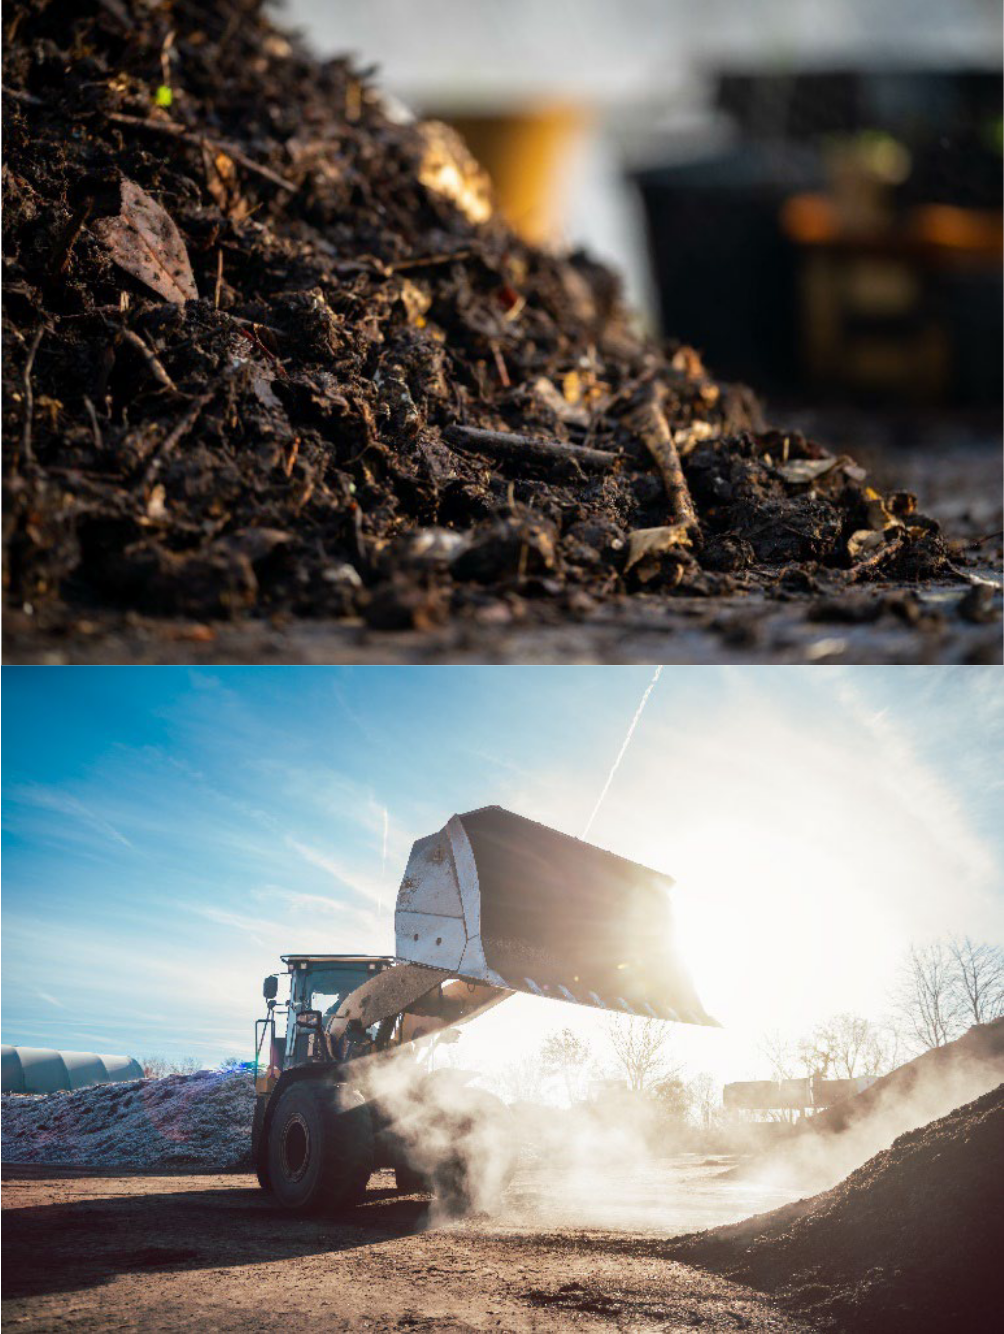
\includegraphics[width=0.6\textwidth]{media/front_practical1.png}\\
\end{center}

\vspace*{1cm}

\setlength{\intextsep}{0pt}%
\begin{wrapfigure}{r}{\textwidth}
    \textbf{\Large Environmental Chemistry and Biology HS2024\\[.5cm]
    \large Dr. Macarena San Martín Ruiz\\
    Lecturer}
    \vspace{-2.1cm}
\end{wrapfigure}

\phantom{}\\[-1cm]

\begin{flushright}
        \large
        \textbf{Team 4}\\
        Matteo Frongillo\\
        Ramadhan Nura\\
        Folagbade Popoola\\
        Jonathan Lawrence Boms\\
        Kron Xhemajli
\end{flushright}
\wrapfill

\tableofcontents
\pagebreak

\section{Composting parameters and plant tolerance test}
\subsection{Introduction}
With this laboratory we will look at the effect of different types of
compost and how it affects the growth of plants. 

Understanding the chemical and physical reactions that occur between
composite materials and plants is essential to developing sustainable
agricultural practices.

\subsection{Materials and methods}
Detail the materials used and the step-by-step procedure followed in the experiment.

\subsection{Results}
\subsubsection{Preliminary parameters}
We collected three samples: Fresh, Finished, and Standard, and 
valuated them based on several characteristics, including pH, color,
texture, odor, foreign objects, and moisture content. Each sample had
distinct features, which helped us assess their condition and quality. 

\renewcommand{\arraystretch}{1.5}
\begin{table*}[ht!]
    \centering \vspace{.3cm}
    \caption{Results of preliminary parameters}
    \hspace*{-.3cm}
    \begin{tabular}{|c|c|c|c|c|c|c|}
        \hline
        \textbf{Sample name} & \textbf{pH} & \textbf{Color} & \textbf{Texture} & \textbf{Odor} & \textbf{Foreign objects} & \textbf{Moisture fist test}\\
        \hline
        Fresh & 9 & Light brown & Coarse & Smells ammonia & -- & 30\% humidity\\
        \hline                                                                   
        \multirow{2}{*}{Finished} & \multirow{2}{*}{8} & \multirow{2}{*}{Dark brown} & \multirow{2}{*}{Fine} & \multirow{2}{*}{Smells ammonia} & Sticks and & \multirow{2}{*}{20\% humidity} \\
                                  &   &            &      &                & plastic particles & \\
        \hline
        Standard & 7 & Darkest brown & Clumpy & Smells earthy & -- & 30\% humidity\\
        \hline
    \end{tabular}
\end{table*}
\phantom{} \vspace*{-.2cm}

\subsubsection{Fresh, Finished and Standard compost}
Three samples were collected, and their raw unit weight was evaluated.
The mass of the empty cylinder was measured in grams, with a value of
168.24 g. The mass of the filled cylinder for each sample was then
measured, obtaining values in liters. The volume of each sample was
also measured in milliliters. Using these measurements, the density
results were calculated in both [kg/L] and [kg/m$^3$] using the formulas:

$\displaystyle \text{Density} \left[kg/L\right] = \frac{\text{Mass of filled cylinder}\ [g] - \text{Mass of empty cylinder}\ [g]}{\text{Volume of sample}\ [mL]}$

$\displaystyle \text{Density} \left[kg/m^3\right] = \text{Density} \left[kg/L\right] \cdot 1000 \left[L/m^3\right]$

The average values provided insight into the consistency of the raw
unit weight across the different samples.


\subsubsection{Fresh compost}
\renewcommand{\arraystretch}{1.5}
\begin{table*}[ht!]
    \centering \vspace{.3cm}
    \caption{Results of raw unit weight in three different samples of fresh compost}
    \begin{tabular}{|c|c|c|c|c|}
        \hline
        \textbf{Sample} & \textbf{1} & \textbf{2} & \textbf{3} & \textbf{Average}\\
        \hline
        {\textbf{Mass of the empty}} & \multicolumn{4}{c|}{\multirow{2}{*}{168.24}}\\
        \textbf{cylinder in [g]} & \multicolumn{4}{c|}{}\\
        \hline
        \textbf{Mass of the filled} & \multirow{2}{*}{120.88} & \multirow{2}{*}{112.20} & \multirow{2}{*}{108.71} & \multirow{2}{*}{113.93}\\
        \textbf{cylinder [g]} & & & &\\
        \hline
        \textbf{Volume of the} & \multirow{2}{*}{340} & \multirow{2}{*}{330} & \multirow{2}{*}{390} & \multirow{2}{*}{353.33}\\
        \textbf{sample in [mL]} & & & &\\
        \hline
        \textbf{Result in [kg/L]} & 0.356 & 0.34 & 0.279 & 0.325\\
        \hline
        \textbf{Result in [kg/m$^3$]} & 356 & 340 & 279 & 325\\
        \hline
    \end{tabular}
\end{table*}

\newpage
\subsubsection{Finished compost}
\renewcommand{\arraystretch}{1.5}
\begin{table*}[ht!]
    \centering \vspace{.3cm}
    \caption{Results of raw unit weight in three different samples of finished compost}
    \begin{tabular}{|c|c|c|c|c|}
        \hline
        \textbf{Sample} & \textbf{1} & \textbf{2} & \textbf{3} & \textbf{Average}\\
        \hline
        {\textbf{Mass of the empty}} & \multicolumn{4}{c|}{\multirow{2}{*}{168.24}}\\
        \textbf{cylinder in [g]} & \multicolumn{4}{c|}{}\\
        \hline
        \textbf{Mass of the filled} & \multirow{2}{*}{214.54} & \multirow{2}{*}{202.91} & \multirow{2}{*}{202.68} & \multirow{2}{*}{206.71}\\
        \textbf{cylinder [g]} & & & &\\
        \hline
        \textbf{Volume of the} & \multirow{2}{*}{375} & \multirow{2}{*}{370} & \multirow{2}{*}{380} & \multirow{2}{*}{375}\\
        \textbf{sample in [mL]} & & & &\\
        \hline
        \textbf{Result in [kg/L]} & 0.572 & 0.548 & 0.533 & 0.551\\
        \hline
        \textbf{Result in [kg/m$^3$]} & 572 & 548 & 533 & 551\\
        \hline
    \end{tabular}
\end{table*}

\subsubsection{Standard compost}
\renewcommand{\arraystretch}{1.5}
\begin{table*}[ht!]
    \centering \vspace{.3cm}
    \caption{Results of raw unit weight in three different samples of standard compost}
    \begin{tabular}{|c|c|c|c|c|}
        \hline
        \textbf{Sample} & \textbf{1} & \textbf{2} & \textbf{3} & \textbf{Average}\\
        \hline
        {\textbf{Mass of the empty}} & \multicolumn{4}{c|}{\multirow{2}{*}{168.24}}\\
        \textbf{cylinder in [g]} & \multicolumn{4}{c|}{}\\
        \hline
        \textbf{Mass of the filled} & \multirow{2}{*}{222.95} & \multirow{2}{*}{228.44} & \multirow{2}{*}{212.74} & \multirow{2}{*}{221.38}\\
        \textbf{cylinder [g]} & & & &\\
        \hline
        \textbf{Volume of the} & \multirow{2}{*}{355} & \multirow{2}{*}{370} & \multirow{2}{*}{360} & \multirow{2}{*}{361.67}\\
        \textbf{sample in [mL]} & & & &\\
        \hline
        \textbf{Result in [kg/L]} & 0.628 & 0.617 & 0.591 & 0.612\\
        \hline
        \textbf{Result in [kg/m$^3$]} & 628 & 617 & 591 & 612\\
        \hline
    \end{tabular}
\end{table*}

\subsection{Experiment results}
\renewcommand{\arraystretch}{1.5}
\begin{table*}[ht!]
    \centering \vspace{.3cm}
    \caption{Experiment results}
    \begin{tabular}{|c|l|l|l|l|l|l|}
        \hline
        \textbf{Group 4} & \textbf{E0} & \textbf{E0} & \textbf{E25} & \textbf{E25} & \textbf{E50} & \textbf{E50} \\
        \hline
        n$^{\circ}$ germinated seeds & 12 & 13 & 11 & 12 & 11 & 10\\
        \hline
        weight (g) & 1.672 & 1.882 & 0.997 & 1.294 & 1.058 & 1.105\\
        \hline
    \end{tabular}
\end{table*}

\vspace*{2cm}
\cfig{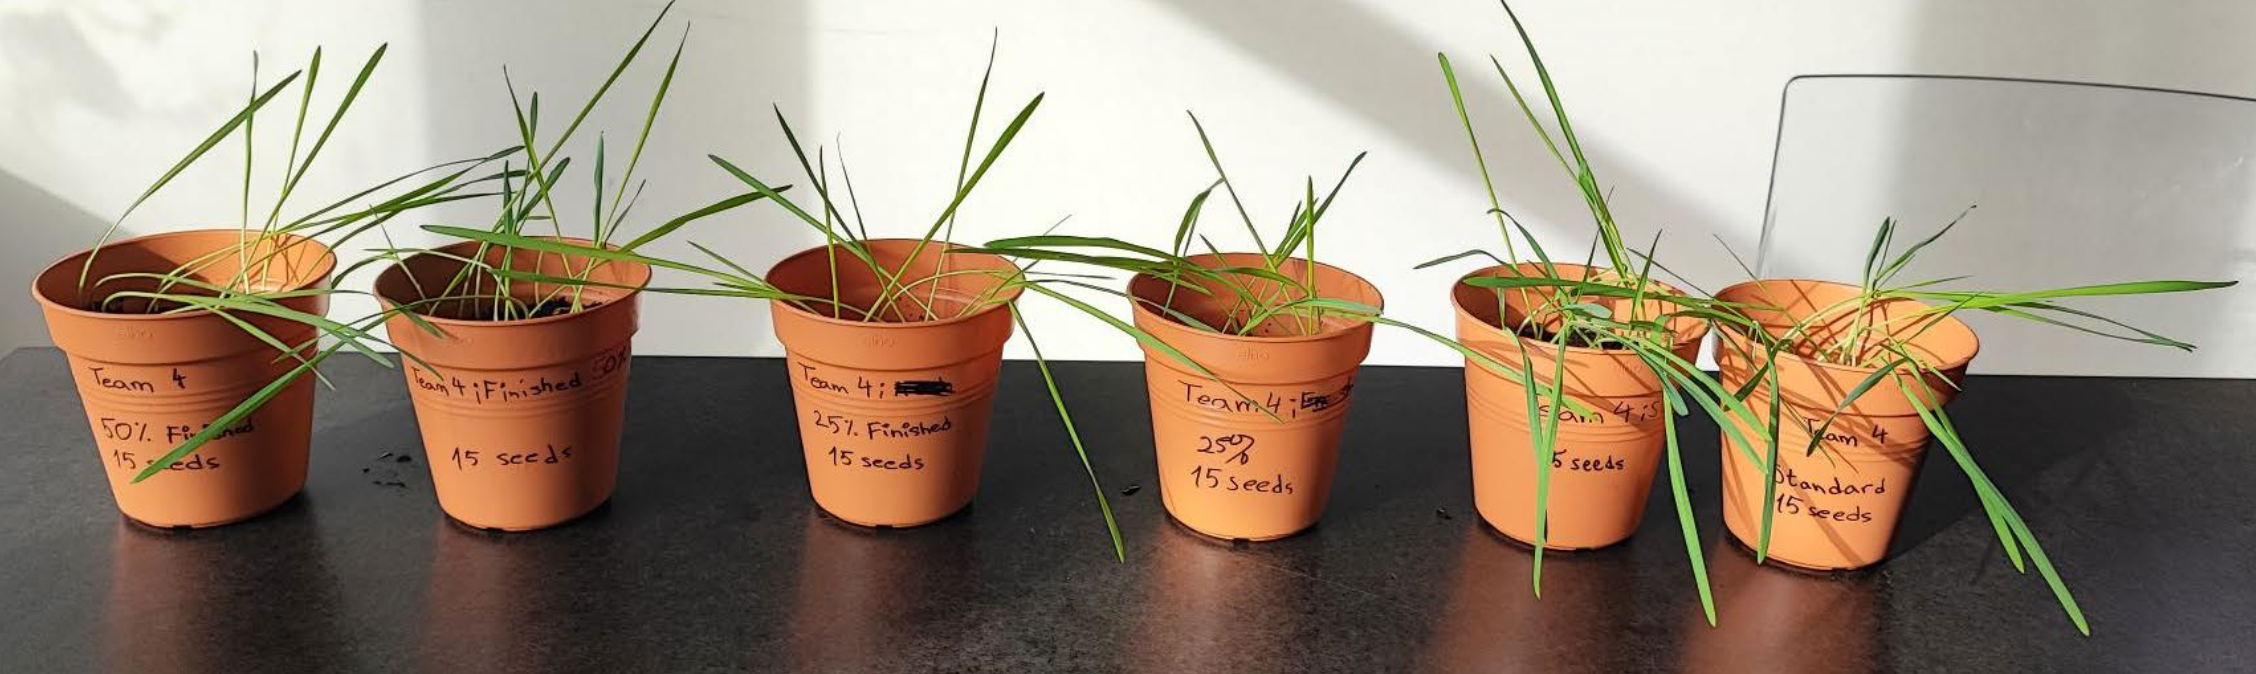
\includegraphics[width=.9\textwidth]{media/plants-results.png}}

\newpage
\subsection{Discussion}
Interpret the results, discussing and answering the questions.

\subsubsection{Results discussion}

\subsubsection{Questions}
\begin{enumerate}
    \item What is the difference between raw unit weight and bulk density? Discuss your
        results based on the laboratory experiment.

        \textbf{R:\\}
            Raw unit weight measures the mass of fresh compost per volume, while
            bulk density includes porosity and moisture. Bulk density is essential for
            assessing aeration and microbial activity, impacting compost structure and
            decomposition efficiency.

    \item How can the pH affect the compost?
    
        \textbf{R:\\}
            pH affects microbial activitiy in composing. Optimal pH (6-8) enhances microbial
            efficiency, while extreme pH values (near 1 or 14) slow down decomposition and
            affect nutrient availability.

    \item What is the impact of immature compost on plant growth, and how can this be
        assessed in the lab?

        \textbf{R:\\}
            Immature compst harms plant growth due to high microbial activity, which
            depletes oxygen and releases toxic substances. In the lab, plant tolerance tests
            measure the compost's effect on germination and growth.

    \item How do you calculate the bulk density of compost, and why is this measurement
        important in the composting process?

        \textbf{R:\\}
            Bulk density is calculated as $\frac{\text{mass}}{\text{volume}}$. It is crucial for
            determining porosity, air flow and moisture retention, directly affecting
            microbial activity and compost quality.

    \item What would be the environmental impact if fresh compost is added in the
        plantations/agriculture or when the recommended percentage of compost mixture
        is not followed?

        \textbf{R:\\}
            Using fresh or excessive compost can release methane, impair growth through
            nitrogen depletion, and cause nutrient leaching, leading to water contamination.

\end{enumerate}

\subsection{Conclusion}
Summarize the key findings and their implications.

\subsection{References}
List any sources or references used for understanding the experiment.

\newpage
\listoftables

\listoffigures






\end{document}
